\section{Theorie}
\label{sec:Theorie}
%%%%%%%%%%%%%%%%%%%%%%%%%%%%%%%%%%%%%%%%%%%%%%%%%%%%%%%%%%%%%%%%%%%%%%%%%%%%%%%%%%%%%%%%%%%%%%%%%%%%%%%%
\subsection{Grundlagen}
\label{sec:Grundlagen}
Atomkerne sind nur für bestimmte Verhältnisse ihrer Bestandteile, den Protonen und Neutronen, stabil.
Bei sogenannten Isotopen ist nun die Protonenanzahl identisch, also handelt es sich um das gleiche 
Element, die Neutronenzahl aber ist verschieden. So sind die Verhältnisse der Protronen und Neutronen
im Atomkern bei verschiedenen Isotopen unterschiedlich, weswegen einige Isotope instabile Atomkerne
besitzen. Diese zerfallen dann radioaktiv.\\
Um die verschiedenen Isotope eindeutig in Fromeln darstellen zu können, wird die Massenzahl des Elements
oben links neben das Elementensymbol geschrieben und gegebenfalls wird auch die Kernladung unten links 
hinzugefügt.\\
Der radioaktive Zerfall ist dabei nicht deterministisch, sodass dieser durch eine Wahrscheinlichkeit 
charakterisiert wird. Diese Zerfallswahrscheinlichkeit kann durch die Halbwertszeit $T$ beschrieben 
werden. Die Halbwertszeit ist dabei die Zeit, in der die Hälte der instabilen Atomkerne zerfallen sind
und kann bei verschiedenen Isotopen um 23 Größenordnungen verteilt sein.\\
%%%%%%%%%%%%%%%%%%%%%%%%%%%%%%%%%%%%%%%%%%%%%%%%%%%%%%%%%%%%%%%%%%%%%%%%%%%%%%%%%%%%%%%%%%%%%%%%%%%%%%%%
\subsection{Gewinnung von Isotopen durch Neutronenbeschuss}
\label{sec:Neutronenbeschuss}
In dem Versuch werden aus praktischen Gründen Isotope mit einer Halbwertszeit zwischen Sekunden und 
wenigen Stunden verwendet. Da diese auf Grund des raschen Zerfalls nicht natürlich vorkommen, werden 
sie vor Beginn der Messung durch Neutronenbeschuss hergestellt. Ein Atom $\ce{^{m}_{z}A}$ wird dabei 
mit einem Neutron $\ce{^{1}_{0}n}$ beschossen und reagiert mit diesem nach
\begin{equation}
    \ce{^{m}_{z}A}+\ce{^{1}_{0}n -> ^{m + 1}_{z}A^* -> ^{m + 1}_{z}A}+\gamma.
    \label{eqn:iso1}
\end{equation}
Das nun entstandene Isotop $\ce{^{m + 1}_{z}A}$ ist dann jenes, welches für das Experiment benötigt
wird. In diesem Fall werden als Ausgangselemente Vanadium-51 und Rhodium-103 verwendet. Die 
Reaktionen lauten also nach \ref{eqn:iso1}:
%Doppelpunkt eher unschön.Alternativen aber auch
\begin{align*}
    \ce{^{51}V}+\ce{^{1}n&->^{52}V}\\
    \ce{^{103}Rh}+\ce{^{1}n}&
    \begin{cases}
        \ce{->[10\%]^{104 i}Rh}\\
        \ce{->[90\%]^{104}Rh}
    \end{cases}
\end{align*}
Rhodium ist insofern ein Spezialfall, dass es in zwei verschiedene isomere Isotope zerfällt. Bei diesen
ist die Anordnung der Kernbausteine verschieden, weswegen sich auch der Verlauf des weiteren Zerfalls
unterscheidet. Der weitere Zerfall wird im folgenden Kaptiel \ref{sec:Zerfallsreaktionen} näher erläutert. 
%%%%%%%%%%%%%%%%%%%%%%%%%%%%%%%%%%%%%%%%%%%%%%%%%%%%%%%%%%%%%%%%%%%%%%%%%%%%%%%%%%%%%%%%%%%%%%%%%%%%%%%
\subsection{Zerfallsreaktionen}
\label{sec:Zerfallsreaktionen}
In diesem Abschnitt werden die Zerfälle der soeben erhaltenen Isotope weiter erläutert.
\subsubsection*{Vanadium-52} 
Der beim Vanadium-52 auftretende Zerall ist ein $\beta^-$-Zerfall. Bei diesem wird im Kern ein Neutron
in ein Proton umgewandelt. Dabei entsteht ein hochenergetisches Elektron $\beta^-$, sowie ein 
Antineutrino $\bar{\nu}_e$. Die Reaktion ist
\begin{equation}
    \ce{^{52}_{23}V -> ^{52}_{24}Cr}+\beta^-+\bar{\nu}_e. 
    \label{eqn:VZerfall}
\end{equation}
\subsubsection*{Rhodium-104 und -104i}
Auch Rhodium-104 ist ein $\beta^-$-Strahler und zerfällt demnach auf die gleiche Art und Weise wie 
Vanadium-52. Die Reaktion ist demnach analog zu \ref{eqn:VZerfall}
\begin{equation}
    \ce{^{104}_{45}Rh -> ^{104}_{46}Pd}+\beta^-+\bar{\nu}_e. 
    \label{eqn:RhZerfall}
\end{equation}
Das isomere Rhodium-104i geht durch die Emission eines $\gamma$-Quantes in Rhodium-104 über.Dieser 
Vorgang wird durch
\begin{equation}
    \ce{^{104 i}Rh -> ^{104}Rh}+\gamma 
    \label{eqn:Rh-104i}
\end{equation}
beschrieben. Das dabei entstehende Rhodium-104 zerfällt dann weiter nach Gleichung \ref{eqn:RhZerfall}.
%%%%%%%%%%%%%%%%%%%%%%%%%%%%%%%%%%%%%%%%%%%%%%%%%%%%%%%%%%%%%%%%%%%%%%%%%%%%%%%%%%%%%%%%%%%%%%%%%%%%%%%%
\subsection{Mathematische Beschreibung}
\label{sec:mathe}
Die Anzahl an den Ausgangskernen $N_0$ nimmt bei radioaktivem Zerfall exponentiell ab. Dabei ist die 
Anzahl $N(t)$ an übrigen Atomen nach der Zeit $t$ gegeben durch das Zerfallsgesetz
\begin{equation}
    N(t)=N_0\text{e}^{-\lambda t} 
    \label{eqn:Zerfallsgesetz}
\end{equation}
mit der Zerfallskonstante $\lambda$. Aus dem Zerfallsgesetz \ref{eqn:Zerfallsgesetz} kann nun die mathematische
Definition der Halbwertszeit hergeleitet werde. Wie in Kapitel \ref{sec:Grundlagen} beschrieben ist die 
Halbwertszeit die Zeit $T$ nach der nurnoch $\frac{1}{2}N_0$ der Kerne übrig sind. Mit Gleichung 
\ref{eqn:Zerfallsgesetz} ergibt sich
\begin{equation*}
    \frac{1}{2}N_0=N_0\text{e}^{-\lambda T}.
\end{equation*}
Daraus folgt 
\begin{equation}
    T=\frac{\ln(2)}{\lambda} 
    \label{eqn:T}.
\end{equation}
Gemessen wird nun jedoch die Zahl der zerfallenen Kerne $N_{\Delta t}(t)$ und nicht die, der noch übrigen
Kerne $N(t)$. $N_{\Delta t}(t)$ ist nun die Differenz zwischen den Kernen $N(t)$ und $N(t+\Delta t)$, 
also
\begin{equation*}
    N_{\Delta t}(t)=N(t)-N(t+\Delta t) 
    \label{eqn:Zerfall1},
\end{equation*}
woraus sich mit Gleichung \ref{eqn:Zerfall1}
\begin{equation*}
    N_{\Delta t}(t)=N_0\text{e}^{-\lambda t}-N_0\text{e}^{-\lambda (t+\Delta t)}
    =N_0(1-\text{e}^{-\lambda \Delta t})\text{e}^{-\lambda t}
\end{equation*}
ergibt. Daraus folgt nach Anwendung des natütlichen Logarithmus 
\begin{equation}
    \ln(N_{\Delta t}(t))
    =\ln(N_0(1-\text{e}^{-\lambda \Delta t}))-\lambda t 
    \label{eqn:Zerfall2}.
\end{equation}
Die Gleichung \ref{eqn:Zerfall2} ist dabei eine Gleichung der Form 
\begin{equation}
    y(t)=a\cdot t+b 
    \label{eqn:gerade}
\end{equation}
mit
\begin{align*}
    y(t)&=\ln(N_{\Delta t}(t))\\
    a&=-\lambda\\
    b&=\ln(N_0(1-\text{e}^{-\lambda \Delta t})).
\end{align*}
Somit lässt sich die Halbwertszeit $T$ mit Gleichung \ref{eqn:T} aus der Zerfallskonstante $lambda$
bestimmen, wobei $\lambda$ durch die negative Steigung der Gerade \ref{eqn:Zerfall2} gegeben ist.
\subsubsection*{Besonderheit bei Isotopengemischen}
Bei Rhodium liegt wie in Kapitel \ref{sec:Neutronenbeschuss} beschrieben ein Isotopengemischen aus 
Rhodium-104 und -104i vor, wobei Rhodium-104i nach Gleichung \ref{eqn:Rh-104i} in Rhodium-104 zerfällt,
welches dann weiter zerfällt. Es laufen demnach gleichzeitig zwei Zerfälle mit unterschiedlicher 
Halbwertszeit ab. Zudem werden durch den Zerfall des Rhodium-104i neue Rhodium-104 Kerne gebildet, sodass
Gleichung \ref{eqn:Zerfall2} nicht mehr gilt.\\
Die Lösung des ersten Problems, also dass gleichzeitig zwei Zerfälle mit unterschiedlichen 
Halbwertszeiten statt finden, folgt aus der Tatsache, dass sich die Halbwertszeiten der beiden Reaktionen
stark unterscheiden. Es gilt nämlich
\begin{align*}
    T_{\ce{^{104}Rh}}>>T_{\ce{^{104i}Rh}}\\
    \Rightarrow
    \lambda_{\ce{^{104}Rh}}<<\lambda_{\ce{^{104i}Rh}}.
\end{align*}
So kann nach einer gewissen Zeit $t^*$ nurnoch der Zerfall von Rhodium-104 beobachtet werden, da das 
Rhodium-104i bereits fast volltändig zerfallen ist. Wenn dieser Umstand in der Ausgleichsrechnung 
mit berücksichtigt wird, können beide Halbwertszeiten der Probe in guter Näherung bestimmt werden.
Der Zerfall einer solchen Probe ist in Abbildung \ref{fig:Isotopengemisch} noch einmal graphisch 
dargestellt. 
\begin{figure}[H]
    \centering
    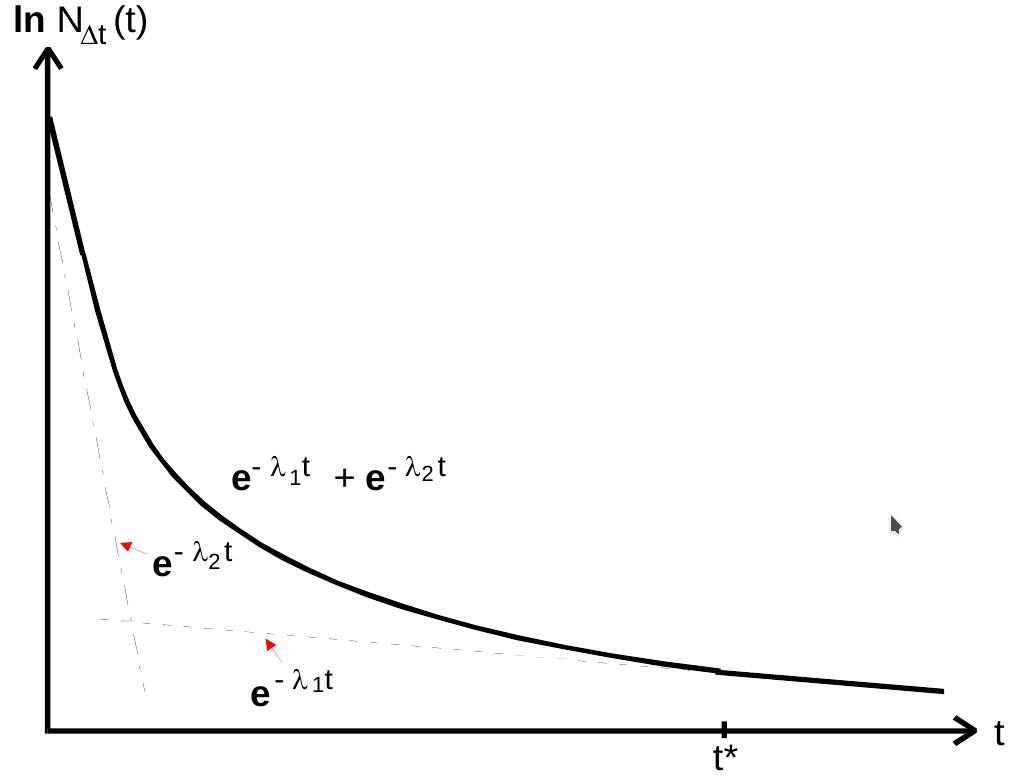
\includegraphics[scale=0.4]{content/Isotopengemisch.png}
    \caption{Zerfallskurve eines Isotopengemisches mit $\lambda_1<<\lambda_2$. Quelle:\cite{AP01}}
    \label{fig:Isotopengemisch}
  \end{figure}
\noindent Das zweite Problem, also dass immer neue Rhodium-104 Kerne geliefert werden, beeinflusst die 
Gesamtbilanz nur sehr gering, weswegen der Effekt vernachlässigt wird. 